\section{Zielsetzung}
\label{sec:zielsetzung}

In dem Versuch werden die Spektren verschiedener $\gamma$-Strahler mit Hilfe
eines Reinst-Germanium-Detektor ausgemessen. Es werden insgesamt vier verschiedene
Proben untersucht. Zu Beginn wird die Theorie hinter der Funktionsweise eines Germanium-Detektors
beschrieben. Danach wird das Vorgehen der Messung erläutert, sowie der Aufbau
skizziert. Anschließend werden die gemessenen Spektren aufgeführt, ausgewertet und
abschließend diskutiert.

\section{Theorie}
\label{sec:theorie}

Im Folgenden wird die Funktionsweise eines Germanium-Detektors beschrieben,
wobei zunächst allgemein die Wechselwirkung von $\gamma$-Quanten mit Materie
betrachtet wird.

$\gamma$-Quanten wechselwirken mit Materie grundlegend über drei verschiedene Effekte,
den Photoeffekt, die Compton-Streuung und die Paarbildung.
Die verschiedenen Effekte haben unterschiedliche Wirkungsquerschnitte $\sigma$,
welche darüberhinaus noch von der Enenergie $E_{\gamma}$ der $\gamma$-Quanten abhängig sind.
Mittels des Wirkungsquerschnittes kann die Größe des Extionsktionskoeffizienten $\mu$
definiert werden. Dieser ist gegeben durch
\begin{equation}
  \label{eqn:ext}
  \mu = n\sigma,
\end{equation}
wobei $n$ die Anzahl der Elektronen pro Volumen $V$ ist.
Der reziproke Extinktionskoeffizient ist die mittlere Reichweite $\bar{x}$
von $\gamma$-Quanten in Materie.
\begin{equation}
  \bar{x} = \frac{1}{\mu}
\end{equation}
Eine Darstelung der auftretenden Extinktionskoeffizienten $\sigma(E_{\gamma})$ ist in
Abblidung~\ref{fig:crosssection} zu finden.

\begin{figure}
  \centering
  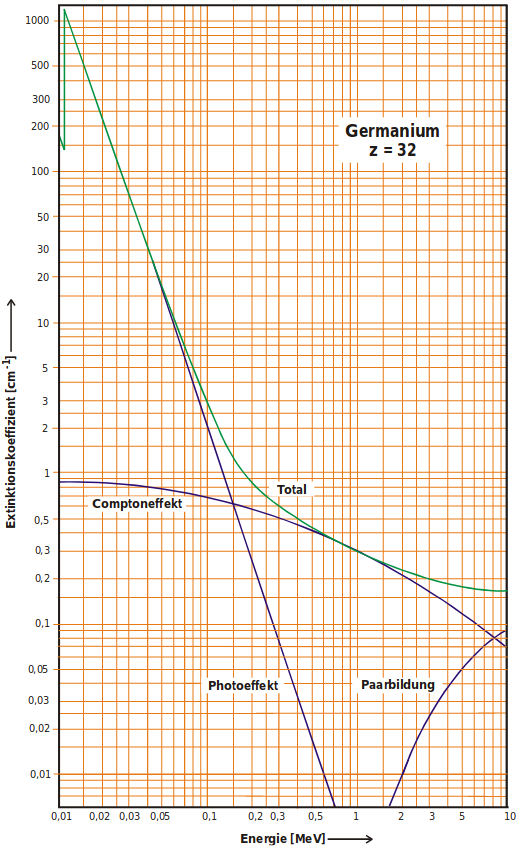
\includegraphics[width=0.8\textwidth]{Pics/crosssection.png}
  \caption{Extinktionskoeffizienten der verschiedenen Wechselwirkungen von $\gamma$-Quanten mit Germanium\cite{anleitung}.}
  \label{fig:crosssection}
\end{figure}

\subsection{Photoeffekt}
\label{subsec:photo}

Der Photoeffekt beschreibt die Wechselwirkung eines $\gamma$-Quantes mit einem
Hüllenelektron der bestrahlten Materie.
Phänomenologisch kann der Photoeffekt über die folgende Gleichung erklärt werden.

\begin{equation}
  \label{eqn:photo}
  \gamma + \ce{Atom -> Atom^+} + e^-
\end{equation}

Somit beschreibt der Photoeffekt die Ionisation eines Atoms.
Das eingehende $\gamma$-Quant besitzt die Energie $E_{\gamma} > E\ua{B}$.
Dabei ist $E\ua{B}$ die Bindungsenergie des Elektrons an dem Atom.
Die Energiedifferenz zwischen $E_{\gamma}$ und $E\ua{B}$ trägt das Elektron in Form
von kinetischer Energie.
Das ausgelöste Elektron hinterlässt in dem Atom ein Loch, welhes durch ein Elektron
aus einer höheren Schale gefüllt wird. Die dabei frei werdende Energie
ist typischer Weise im Bereich der Röntgenstrahlung. In guter Näherung kann angenommen
werden, dass diese Röntgen-Quanten den Absorber nicht verlassen.
Das bedeutet bei dem Photoeffekt ist davon auszugehen, dass die vollständige
Energie des $\gamma$-Quantes im Absorber verbleibt.

Der Wirkungsquerschnitt des Photoeffektes ist für den in dem Versuch auftretenden
Energieberich approximativ mit
\begin{equation}
  \label{eqn:crosssection_photo}
  \sigma\ua{Ph} \sim \frac{z^\alpha}{E^{\num{3,5}}}
\end{equation}
gegeben. $z$ entspricht der Kernladungszahl der wechselwirkenden Materie und $\alpha$
ist eine Exponent mit $4 < \alpha < 5$~\cite{anleitung}.

\subsection{Compton-Streuung}
\label{subsec:compton}

Der Compton-Effekt beschreibt die Streuung von $\gamma$-Quanten an freien Elektronen
und wird durch folgende Gleichung beschrieben.

\begin{equation}
  \label{eqn:compton}
  \gamma + e^- \ce{->} \gamma '+ (e^-)'
\end{equation}

Gleichung~\eqref{eqn:compton} sagt aus, dass ein Energieübertrag zwischen dem
$\gamma$-Quant und dem Elektron $e^-$ stattfindet.
Der Prozess ist in Abbildung~\ref{fig:compton} schematisch illustriert.

\begin{figure}
  \centering
  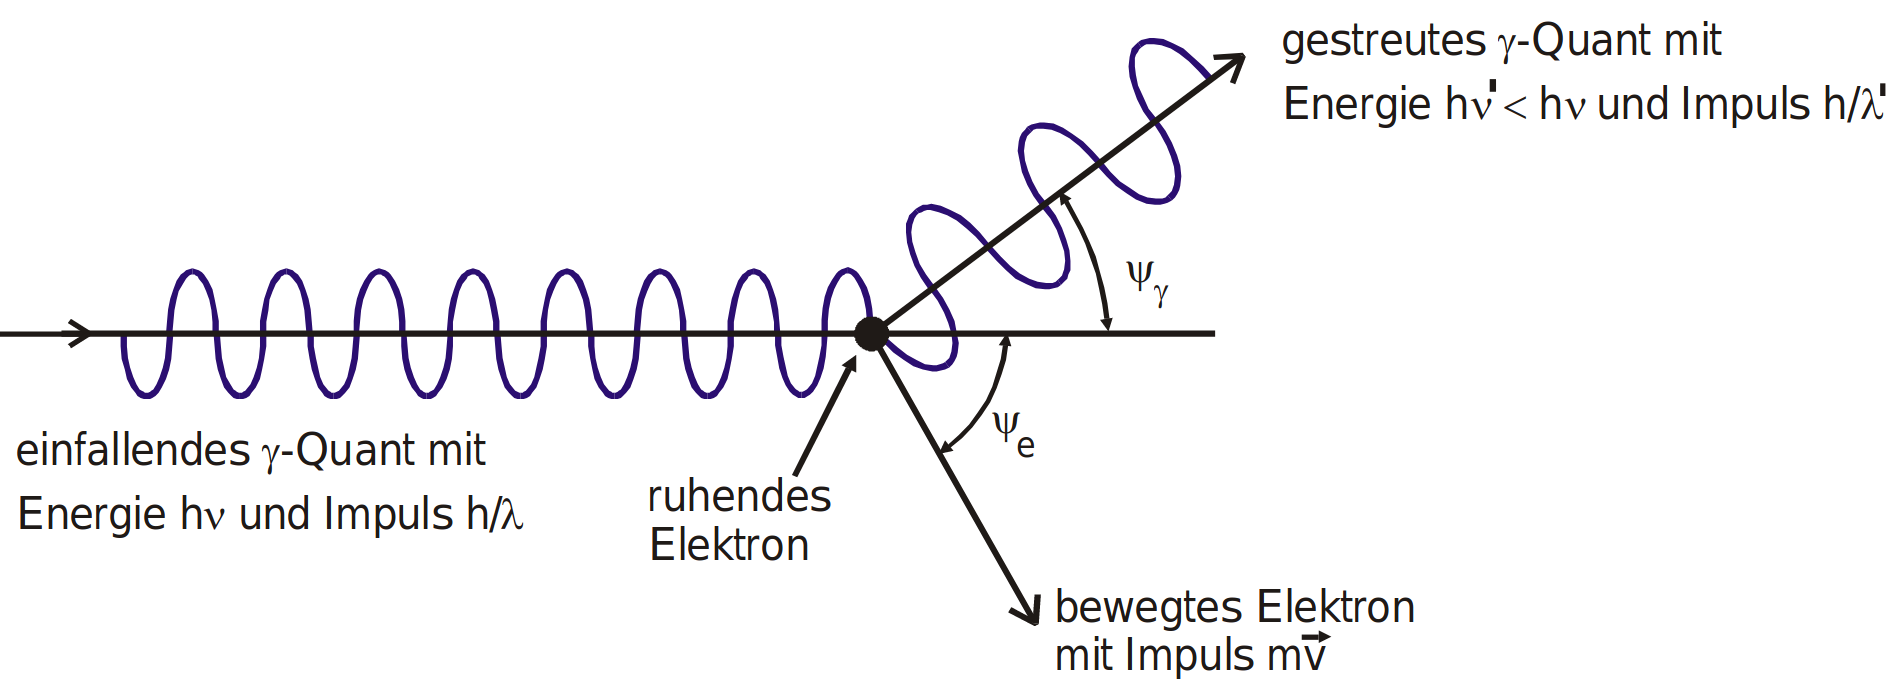
\includegraphics[width=0.8\textwidth]{Pics/compton.png}
  \caption{Schematische Darstellung der Compton-Streuung. $\Psi_\gamma$ ist der Streuwinkel des
  $\gamma$-Quantes und $\Psi_{e^-}$ ist der Streuwinkel des gestoßenen Elektrons\cite{anleitung}.}
  \label{fig:compton}
\end{figure}

Die Impuls- und Energieerhlatung eines inelastischen Stoßen führen auf eine
$\gamma$-Quantenergie nach der Streuung $E_{\gamma}'$ von
\begin{equation}
  \label{eqn:comton_E_gamma}
  E_\gamma ' = E_\gamma\frac{m_0c^2}{m_0c^2 + E_\gamma\left(1 - \cos{(\Psi_\gamma)}\right)}.
\end{equation}
Die Energie des Elektrons nach der Streuung $E_{e^-}'$ ist gegeben durch
\begin{equation}
  \label{eqn:comton_E_el}
  E_{e^-}' = E-\gamma - E_\gamma ' = \frac{E_\gamma^2\left(1 - \cos{(\Psi_\gamma)}\right)}{m_0c^2 + E_\gamma\left(1 - \cos{(\Psi_\gamma)}\right)}.
\end{equation}
Der maximale Energieübertrag ist somit gegeben für $Psi_\gamma = \SI{180}{\degree}$,
was einer Rückstreuung entspricht. Der Bereich Streuung bei diesem Streuwinkel wird
im Energiespektrum als Compton-Kante bezeichnet (vgl. Kapitel~\ref{subsec:energiespektrum}).

\subsection{Paarbildung}
\label{subsec:paar}

Die Paarbildung tritt erst ab einer $\gamma$-Quantenergie von $E\gamma > 2m_0c^2$
auf, weshalb sie bei der hier betriebenen $\gamma$-Spektroskopie keinen
Einfluss hat. Der Prozess kann durch eine Gleichung der Form
\begin{equation}
  \label{eqn:paar}
  \gamma + \ce{Atom -> Atom} + e^+ + e^-
\end{equation}
erklärt werden. Aus Impulserhaltungsgründen ist die Energie des $\gamma$-Quantes
auf beide Leptonen gleimäßig aufgeteilt.
Anstelle des Atoms in~\ref{eqn:paar} kann auch ein Elektron als Stoßpartner
fungieren, wobei die Paarbildung an Elektronen aufgrund einer höheren Schwellenenergie,
welche aus der geringeren Masse resultiert, unwahrscheinlicher ist.
Es wird nicht in jedem Fall die gesamte Energie eines einfallenden $\gamma$-Quantes
im Absorber deponiert. Das erzeugte Positron rekonbiniert mit einem Elektron
des Absorbers, wobei aus Impulserhaltungsgründen zwei Photonen entstehen.
Mit einer endlichen Wahrscheinlichkeit kann eines der beiden, oder sogar beide
Photonen nicht wieder mit dem Absorber wechselwirken und
den Detektor ohne Energiedeponierung verlassen.

\subsection{Wirkungsweise eines Reinst-Germanium-Detektors}
\label{subsec:wirkungsweise}
Germanium ist ein indirekter Halbleiter, weshlab ein Reinst-Germanium-Detektor
zu den Halbleiter-Detektoren gezählt wird.
